\begin{figure}[hp]
    \centering
    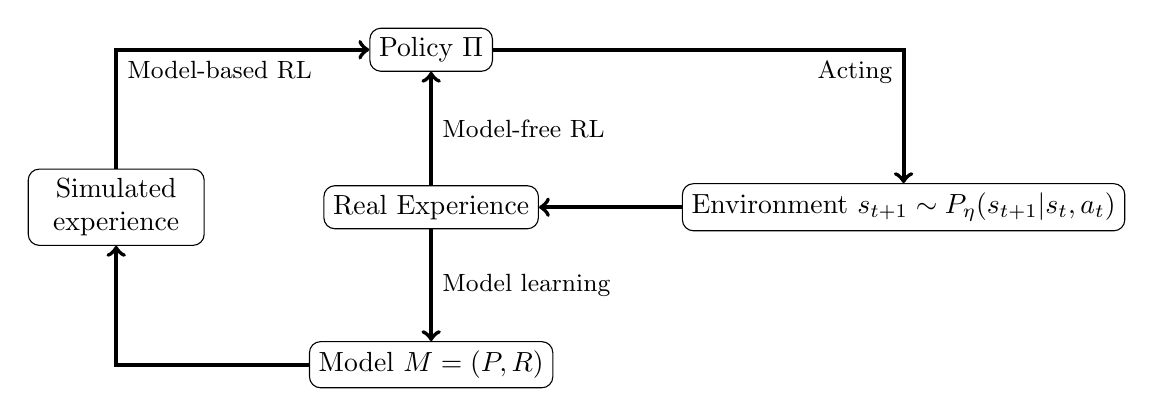
\begin{tikzpicture}[node distance=2cm]
        % Define nodes
        \node (policy) [rounded corners, draw] {Policy $\Pi$};
        \node (real_experience) [rounded corners, draw, below of=policy] {Real Experience};
        \node (environment) [rounded corners, draw, right of=real_experience, node distance=6cm] {Environment $s_{t+1}\sim P_\eta(s_{t+1}|s_t, a_t)$};
        \node (model) [rounded corners, draw, below of=real_experience] {Model $M = (P,R)$};
        \node (simulated_experience) [align=center, text width=2cm, rounded corners, draw, left of=real_experience, node distance=4cm] {Simulated experience};
        
        % Draw arrows
        \draw[->, line width=1.5pt] (policy) -| (environment) node[midway, below left, font=\small] {Acting};
        \draw[->, line width=1.5pt] (environment) -- (real_experience);
        \draw[->, line width=1.5pt] (real_experience) -- (model) node[midway, right, font=\small] {Model learning};
        \draw[->, line width=1.5pt] (model) -| (simulated_experience);
        \draw[->, line width=1.5pt] (real_experience) -- (policy) node[midway, right, font=\small] {Model-free RL};
        \draw[->, line width=1.5pt] (simulated_experience) |- (policy) node[font=\small, midway, below right] {Model-based RL};
    \end{tikzpicture}
    \caption{Model-free \ac{RL} vs. Model-based \ac{RL}}
    \label{fig:demo}
\end{figure}
% \tikzstyle{block} = [draw, fill=white, rectangle, 
%     minimum height=3em, minimum width=6em]
% \tikzstyle{sum} = [draw, fill=white, circle, node distance=1cm]
% \tikzstyle{input} = [coordinate]
% \tikzstyle{output} = [coordinate]
% \tikzstyle{pinstyle} = [pin edge={to-,thin,black}]

% \begin{tikzpicture}[auto, node distance=2cm,>=latex']

%     \node [input, name=input] {};
%     \node [sum, right of=input] (sum) {};
%     \node [block, right of=sum] (controller) {Controller};
%     \node [block, right of=controller, pin={[pinstyle]above:D},
%             node distance=3cm] (system) {System};

%     \draw [->] (controller) -- node[name=u] {$u$} (system);
%     \node [output, right of=system] (output) {};
%     \node [block, below of=u] (measurements) {Measurements};

%     \draw [draw,->] (input) -- node {$r$} (sum);
%     \draw [->] (sum) -- node {$e$} (controller);
%     \draw [->] (system) -- node [name=y] {$y$}(output);
%     \draw [->] (y) |- (measurements);
%     \draw [->] (measurements) -| node[pos=0.99] {$-$} 
%         node [near end] {$y_m$} (sum);
% \end{tikzpicture}
